%\documentclass{beamer}

\documentclass[hyperref={unicode}]{beamer}
\usepackage{kotex}
\usepackage[ps]{hfontsel}

%\usepackage{kotex}
\usepackage{hyperref}
%\usepackage{multirow}
\usepackage{graphicx}
\usepackage{amssymb,amsfonts,amsmath}
\usepackage{enumerate}
% \usepackage{setspace}
%\onehalfspacing


%\usetheme{Madrid} % Beamer theme v 3.0
  \setbeamertemplate{background canvas}[vertical shading][bottom=red!10,top=blue!10]
\usetheme{Warsaw}
 \usefonttheme[onlysmall]{structurebold}
%\usecolortheme{lily} % Beamer color theme
\setbeamercovered{dynamic}

\begin{document}

\author{조남운\\ \url{mailto:namun.cho@gmail.com}}
\title{프리젠테이션을 위한 Beamer class}
\date{2008.2.20}

\begin{frame}
  \titlepage
\end{frame}


%\chapter{프리젠테이션용 파일 만들기}\label{ch:presentation}
%\LaTeX를 프리젠테이션에 사용할 수 있다. 프리젠테이션을 위해 만들어진 문서 클래스가 바로 Beamer class이다. 가장 간단하게는 단지 documentclass를 beamer로 지정하기만 하면 된다. 하지만 그렇게 할 경우 프리젠테이션에 그리 적당한 문서가 나오지 않는다. 따라서 beamer 클래스에써 제공하는 특수한 명령어를 통해 프리젠테이션에 적당한 문서를 만드는 것이 좋다. 자세한 내용은 beamer manual(\url{http://mixing.coas.oregonstate.edu/links/latex_files/beamer.pdf})을 참조하도록 하라. 

\section{frame 환경}
%beamer 클래스에서 각 장은 프레임이라고 부르며, 이 프레임의 시작과 끝은 \verb!\begin{frame}!과 \verb!\end{frame}!으로 정해진다. 타이틀 페이지는 다음과 같이 만들 수 있다. 

\begin{frame}[fragile]
\begin{block}{frame환경}<1->
\begin{itemize}
  \item 프레임 : 프리젠테이션을 구성하는 한 면을 의미
  \item 한 프레임을 구성하는 실제 결과물은 여러 장이 될 수 있음(애니메이션)
\end{itemize}
\begin{block}{제목을 나타내는 프레임의 예}<2->
\begin{verbatim}
  \begin{frame} 
    \maketitle % same as : \titlepage
  \end{frame} 
\end{verbatim}
\end{block}
\end{block}
\end{frame}



\begin{frame}[fragile]
%itemize같은 환경은 프레임 내에서 시작해서 끝나야만 한다. 따라서 부득이하게 하위 item을 이어서 해야 할 경우, \verb!\item[]!을 이용하여 하위 아이템으로 시작한 듯 보이게 해야 한다. 

\begin{columns}[c]
\begin{column}{0.5\textwidth}
\begin{block}{itemize환경의 연결}
\tiny
\begin{center}
\begin{verbatim}
  \begin{frame}
    \begin{itemize}
      \item 1차 item
      \begin{itemize}
        \item 2-1 item
        \item 2-2 item 
      \end{itemize}
    \end{itemize}
  \end{frame}

  \begin{frame}
    \begin{itemize}
      \item[]   %%% unobservable 
      \begin{itemize}
        \item 2-3 item
      \end{itemize}
    \end{itemize}
  \end{frame}
\end{verbatim}
\end{center}
\end{block}
\end{column}

\begin{column}{0.5\textwidth}
\begin{center}
	\includegraphics[bb=0 0 262 601, width=0.5\textwidth]{picture_21.ps}
\end{center}
\end{column}

\end{columns}

\end{frame}

%또한, 장, 절 같은 경우 frame 환경 밖에서 설정해야만 한다. 

\begin{frame}[fragile]

\begin{block}{주의사항}
\begin{itemize}
	\item 장, 절 등의 명령은 frame환경 밖에서 선언해야 한다. 
\end{itemize}


\begin{block}{}
\begin{center}
\begin{verbatim}
  \chapter{Beamer class} 
    \section{Basic usuage}

  \begin{frame} 
    장(chapter), 절(section) 등은 frame환경 밖에서 선언해야 합니다!
  \end{frame}

\end{verbatim}
\end{center}

\end{block}
\end{block}
\end{frame}

%프레임의 타이틀은 \verb!\frametitle{프레임 제목}! 명령어를 사용한다. 목차는 \verb!\tableofcontents!를 이용한다. 
\section{block환경}
\begin{frame}[fragile]
\begin{block}{}지금 쓰고 있는 글상자가 바로 block환경이다. \end{block}
\begin{columns}[c]
	\begin{column}{0.5\textwidth}
		\begin{block}{block환경}
			\begin{center}
			\begin{verbatim}
				\begin{block}{이것이 바로 block환경}
				   	이것이 바로 block환경의 내용
				\end{block}
			\end{verbatim}
			\end{center}

		\end{block}	
	\end{column}
	
	\begin{column}{0.5\textwidth}
		\begin{block}{이것이 바로 block환경}
			이것이 바로 block환경의 내용
		\end{block}	
	\end{column}

\end{columns}
\end{frame}

\section{다단 편집}


\begin{frame}[fragile]
%오른쪽에 그림을, 왼쪽에 내용을 나타내게 하고 싶을 경우, columns환경을 사용한다. columns 환경을 통해 총 단의 수를 정하며, 각 단은 column환경을 사용하여 나타낸다. 

\begin{columns}[t]
\begin{column}{0.5\textwidth}
\begin{block}{}
\begin{center}
\begin{verbatim}
  \begin{columns}[옵션]
    \begin{comumn}{사이즈}
    \end{column}
    \begin{column}{사이즈}
    \end{column}
  \end{columns} 
\end{verbatim}
\end{center}
\end{block}%columns 환경의 옵션은 b, c, t, T 등이 있다. 각각 칼럼의 정렬을 바닥, 가운데, 꼭대기로 하는 것을 의미한다. 
\end{column}

\begin{column}{0.5\textwidth}
\begin{itemize}
\item 다단 편집에는 columns와 column환경을 사용
\item columns환경 안에 column환경이 둘러싸여 있는 형식을 사용함. 
\end{itemize}

\end{column}

\end{columns}
\end{frame}

\begin{frame}[fragile]
\begin{block}{}
\tiny

\begin{verbatim}
  \begin{columns}[t] 
    \begin{column}{0.5\textwidth} 
      Two\\lines. 
    \end{column} 
  
    \begin{column}{0.5\textwidth} 
      One line (but aligned). 
    \end{column} 
  \end{columns} 
  Example: 
  \begin{columns}[t] 
    \begin{column}{0.3\textwidth} 
      Two\\lines. 
    \end{column}
    \begin{column}[T]{0.7\textwidth} 
    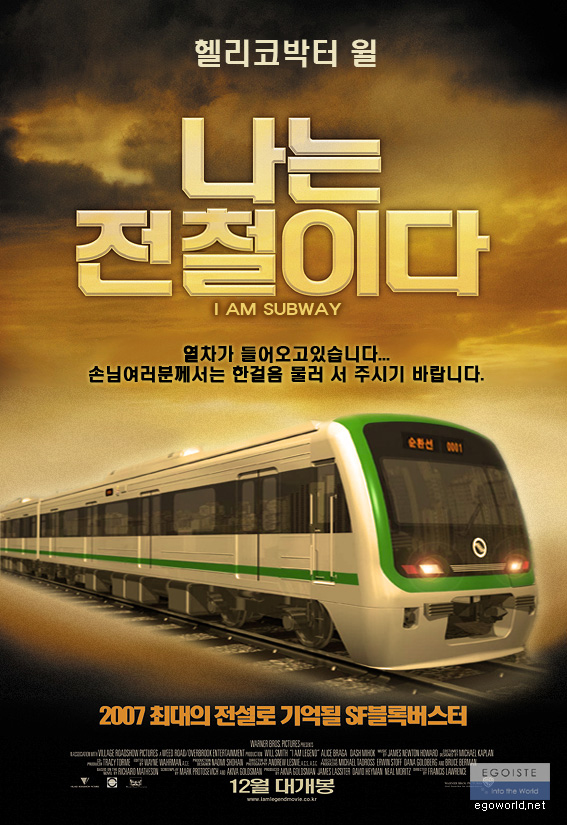
\includegraphics[bb= 0 0 567 825, height=3cm]{abcd.ps} 
    \end{column}
  \end{columns} 
\end{verbatim}
\end{block}
\end{frame}


\begin{frame}
\begin{block}{}
  \begin{columns}[t] 
    \begin{column}{0.3\textwidth} 
      Two\\lines. 
    \end{column} 
  
    \begin{column}{0.3\textwidth} 
      One line (but aligned). 
    \end{column} 
  \end{columns} 
  
  Example: 
  
  \begin{columns}[c] 
    \begin{column}{0.1\textwidth} 
      Two\\lines. 
    \end{column}
    \begin{column}{0.5\textwidth} 
    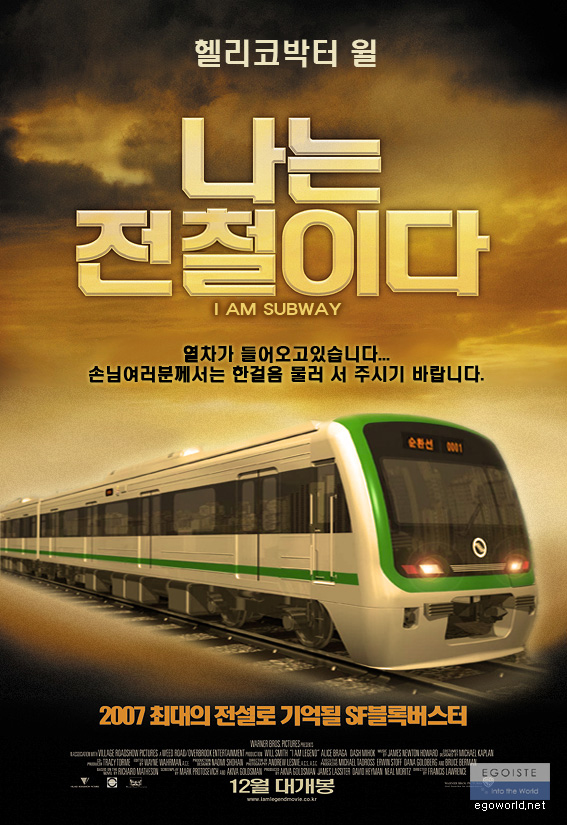
\includegraphics[bb= 0 0 567 825, height=3cm]{abcd.ps} 
    \end{column}
  \end{columns} 
\end{block}
\end{frame}

\section{클릭 순서 편집}

%마우스 클릭을 할때마다 항목이 순차적으로 나타나게 할 수 있다. 실제로는 클릭 수 만큼의 beamer class 문서를 생성하여 마치 클릭 할 때마다 항목이 나타나는 것처럼 보이게 하는 것이다. %비머 클래스의 결과문은 따로 파일을 생성해서 보여줄 것.

\begin{frame}[fragile]
\frametitle{클릭 순서대로 글이 나타나게 하기}

\begin{block}{}
  아래의 프레임을 실행시키면 $<NUM->$의 $NUM$ 순서대로 나타나게 된다. 
\end{block}

\begin{block}{}
\tiny
 \begin{center}
 \begin{verbatim}
  \begin{frame} 
    \frametitle{There Is No Largest Prime Number} 
    \framesubtitle{The proof uses \textit{reductio ad absurdum}.} 
    \begin{block}{Theorem} 
      There is no largest prime number. 
    \end{block} 
    \begin{block}{Proof} 
      \begin{enumerate} 
        \item<1-> Suppose $p$ were the largest prime number. 
        \item<2-> Let $q$ be the product of the first $p$ numbers. 
        \item<3-> Then $q + 1$ is not divisible by any of them. 
        \item<1-> Thus $q + 1$ is also prime and greater than $p$. QED
      \end{enumerate} 
    \end{block} 
  \uncover<4->{The proof used \textit{reductio ad absurdum}.} 
  \end{frame} 
 \end{verbatim}
 \end{center}
\end{block}

\end{frame}

 \begin{frame} 
    \frametitle{There Is No Largest Prime Number} 
    \framesubtitle{The proof uses \textit{reductio ad absurdum}.} 
    \begin{block}{Theorem} 
      There is no largest prime number. 
    \end{block} 
    \begin{block}{Proof} 
      \begin{enumerate} 
        \item<1-> Suppose $p$ were the largest prime number. 
        \item<2-> Let $q$ be the product of the first $p$ numbers. 
        \item<3-> Then $q + 1$ is not divisible by any of them. 
        \item<1-> Thus $q + 1$ is also prime and greater than $p$. QED
      \end{enumerate} 
    \end{block} 
  \uncover<4->{The proof used \textit{reductio ad absurdum}.} 
  \end{frame}


\section{테마와 색상 설정}
\begin{frame}
\begin{block}{}
beamer 클래스에서는 다양한 테마와 색상을 제공한다. 자세한 내용은 beamer class문서를 참고하도록 한다. 
\url{http://faq.ktug.or.kr/wiki/uploads/Beamer/BeamerTheme.pdf}
\end{block}
\end{frame}

\section{노트 출력}
\begin{frame}[fragile]
\begin{itemize}
\item [] 노트로 출력하고 싶은 경우 document class에 옵션으로 `handout'을 넣어준다. 이렇게 하면 클릭 순서 편집으로 인해 늘어난 면을 한 면으로 맞추어 준다. 
\end{itemize}

\begin{block}{}
\begin{verbatim}
  \documentclass[handout]{beamer}
\end{verbatim}
\end{block}

%노트로 출력하고 싶은 경우 document class에 옵션으로 `handout'을 넣어준다. 이렇게 하면 클릭 순서 편집으로 인해 늘어난 면을 한 면으로 맞추어 준다. 칼라 수를 줄이고 싶다면 테마를 바꾸어 준다.
\end{frame}

\begin{frame}
\begin{block}{}
\begin{center}
\Huge
수고하셨습니다!
\end{center}
\end{block}
\end{frame}

\end{document}